\documentclass{article}

% Language setting
% Replace `english' with e.g. `spanish' to change the document language
\usepackage[english]{babel}

% Set page size and margins
% Replace `letterpaper' with `a4paper' for UK/EU standard size
\usepackage[letterpaper,top=2cm,bottom=2cm,left=3cm,right=3cm,marginparwidth=1.75cm]{geometry}

% Useful packages
\usepackage{amsmath}
\usepackage{graphicx}
\usepackage[colorlinks=true, allcolors=blue]{hyperref}
\DeclareMathOperator{\Var}{Var}
\DeclareMathOperator{\E}{E}
\DeclareMathOperator{\Prob}{Prob}
\DeclareMathOperator{\max}{max}
\DeclareMathOperator{\drift}{drift}


\title{Quantitative Models for Options Pricing}
\author{Fabian Farestam, typeset by Om Gupta}
\date{September 2022}

\begin{document}
\maketitle

\section{Introduction}

This document is an overview of quantitative models for option pricing to be implemented in OpenBBTerminal. When learning about options pricing, I recommend you to start with learning the Cox-Ross-Rubinstein Binomial model, then Black-Scholes model and later on advance to more complicated models. \\
Note that none of this is my (Fabian Farestam’s) research. It’s just a reformulation and a collection of material from multiple sources.

\section{Cox-Ross-Rubinstein Binomial Model}

The binomial pricing model has a simple concept, namely that it builds a tree of possible pricing with a certain amount of steps until the time of the options maturity and calculates the arbitrage free price based on this tree. It’s easy to implement (can be $O(2^{n}$)) and also very practical while clearly demonstrating the no arbitrage argument. In special limiting cases of this we can get both the Black-Scholes model as well as the Cox-Ross jump process model (similar to the hybrid jump diffusion model by Merton). \\
The model assumes that:

\begin{itemize}
    \item The stock price follows a multiplicative binominal process over discrete periods
    \item The interest rate is constant and one might borrow and lend as much as wished at this interest rate. (For convenience we assume that r > 1)
\end{itemize}

\subsection{Notation}
\begin{itemize}
    \item $u$: Asset return with the probability of q 
    \item $d$: Asset return with the probability of 1 - q
    \item $S$: Stock Price
    \item $q$: Probability of tree path taken
    \item $r$: Riskless interest rate
    \item $C$: Value of a call option
    \item $K$: Strike Price
\end{itemize}

\subsection{One Step Tree}
The setup is simple, the stock returns over each period is either $u - 1$ with the probability of $q$, or $d - 1$ with the probability $1 - q$. Thus the price at the end of the period will be $uS$ or $dS$. Note that the relation $u > r > d$ must always be held. An illustration of this is:

\begin{figure}
\centering
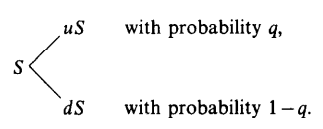
\includegraphics[width=0.3\textwidth]{one-step-tree.png}
\caption{\label{fig:onestep}Source: Cox, Ross, Rubinstein}
\end{figure}

To calculate the value of this simple setup, where there’s only one step, we use:
\begin{align*}
    C_{u} = \max(0, uS - K) \\
    C_{d} = \max(0, dS - K)
\end{align*}
When using a number of shares, $g$ (some use $\delta$ instead of g) and dollar invested in riskless bonds, $B$. Thus:
\begin{align*}
    C_{u} = g u S + r B \\
    C_{d} = g d S + r B 
\end{align*}
After solving for $g$ and $B$,
\begin{align}\label{eq:1}
    \begin{split}
    g = \frac{C_{u} - C_{d}}{(u - d)S} \\
    B = \frac{uC_{d} - dC_{u}}{(u - d)r}
    \end{split}
\end{align}
If no arbitrage exists then:
\begin{equation*}
    C = gS +B
\end{equation*}
Which then implies
\begin{equation}\label{eq:2}
    C = \frac{p C_{u} + (1 - p) C_{d}}{r}
\end{equation}
where $p=\frac{r-d}{u-d}$ and $1-p=\frac{u-r}{u-d}$ \\ [5ex]
From \ref{eq:2} we can make three observations:
\begin{enumerate}
    \item $q$ is not used, thus even if investors have different opinions about the probabilities they can still agree to this relationship! ($p$ is $q$ if investors were to be risk neutral)
    \item Investor’s risk attitude doesn’t matter.
    \item The stock price is the only random variable.
\end{enumerate}
\subsection{Two Step Tree}
For a two step tree we get the following structure:\\
\begin{figure}
\centering
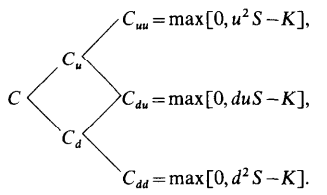
\includegraphics[width=0.3\textwidth]{two_step_tree.png}
\caption{\label{fig:twostep}Source: Cox, Ross, Rubinstein}
\end{figure}
To this new tree we adapt \ref{eq:2}
\begin{align}\label{eq:3}
    \begin{split}
    C_{u} = \frac{p C_{uu} + (1-p) C_{ud}}{r} \\
    C_{d} = \frac{p C_{du} + (1-p) C_{dd}}{r}
    \end{split}
\end{align}
We don't need to change \ref{eq:1}  but just we need to adjust our hedge portfolio with the new values gotten from \ref{eq:3} \\
So to get the value of the call we substitute \ref{eq:3} into \ref{eq:2}, which results in:
\begin{align}\label{eq:4}
    \begin{split}
    C & = \frac{p^{2} C_{uu} + 2 p (1 - p)  C_{ud} + (1 - p)^{2}  C_{dd}}{r} \\
    & = \frac{p^{2}*\max(0, u^{2}S - K) + 2 p (1 - p) * \max(0, duS - K)}{r}
    \end{split}
\end{align}
From this we conclude that all assumptions made from \ref{eq:2} also hold for \ref{eq:4}. Now the list of variables that determine $C$ is $S, K, n, u, d$ and $r$.
\subsection{Binomial tree with any amount of steps}
We can find the call value recursively, by starting at the expiration and working backwards, for any amount of steps:
\begin{equation}\label{eq:5}
    C = \frac{\sum_{j=0}^{n} {n \choose j} p^{j}(1-p)^{n-j}\max(0, u^{j}d^{n-j}S - K)}{r^{n}}
\end{equation}
We’re not yet done since we can express this in a way nicer form by some transformations:
\begin{equation}\label{eq:6}
    C = \frac{\sum_{j=a}^{n} {n \choose j} p^{j}(1-p)^{n-j} (u^{j}d^{n-j}S - K)}{r^{n}}
\end{equation}
where $a$ (represents minimum stock upwards moves for finishing in the money) is the smallest non negative larger greater than $\frac{\log(K / S d^{n})}{\log(u / d)} $ \\
We'll break up the above formula into two terms:
\begin{equation}\label{eq:7}
    C = S *\frac{\sum_{j=a}^{n} {n \choose j} p^{j}(1-p)^{n-j} (u^{j}d^{n-j})}{r^{n}} - K * \frac{\sum_{j=a}^{n} {n \choose j} p^{j}(1-p)^{n-j}}{r^{n}}
\end{equation}
In formula \ref{eq:7} we have two brackets, when taking a closer look at them one realises that we can express them as complementary binomial distribution function $\phi$. We can sum this up as the final simple Binomial Pricing formula:
\begin{equation}\label{eq:8}
    C = S *\phi(a; n, p) - K r^{-n} * \phi(a; n, p')
\end{equation}
where $p=\frac{r-d}{u-d}$ and $p'=\frac{u}{r}p$\\ [2ex]
Note that the formula above is only valid for American non-dividend paying call options.
\subsection{Dividends}
In this part in order to account for the dividend we assume that the stock has a constant dividend yield, $\delta$ on the ex-dividend date and a total of $v$ ex-dividend days. To account for dividend we need to define $\rho$ as one plus the interest rate over a period of $h=\frac{t}{n}$. The total return  is $\rho^{n} = r^{t}$, and we can express $\rho= r^{\frac{t}{n}}$. \\
A major difference in this model “extension“ is that early exercise is optimal in some cases. Early exercise is in fact optimal when $S > S^{*}$, where $S^{*}$ is the “critical” price of the stock where the following equation holds:
\begin{equation}\label{eq:9}
    S^{*} - K = \frac{p*C(n,i-1,j+1) + (1-p)*C(n,i-1,j)}{\rho}
\end{equation}
for $j = 0, 1, 2, .., n-i$ where $C(n, i, j) =$ call value $n-i$ periods from now, $S^{*} = u^{j}d^{n-i-j}(1-\delta)^{v(n,1)}*S$, and $v(n,i)=\sum_{k=1}^{n-1}v_{k}$ \\ [4ex]
From \ref{eq:9}, we get 
\begin{equation}\label{eq:10}
   C(n,i,j) = \max\left(u^{j}d^{n-i-j}(1-\delta)^{v(n,1)}*S - K, \frac{p*C(n,i-1,j+1) + (1-p)*C(n,i-1,j)}{\rho}\right)
\end{equation}
Important to note is that here we traverse the price the binomial tree recursively, thus starting with $i = 0$ and ending with $i = n$. We apply the previous results into the calculations of the previous ones. \\ [2ex]
The hedge ratio of the portfolio is:
\begin{equation*}
    g = \frac{C(n, n - 1, 1) - C(n, n -1, 0)}{(u - d) * S}
\end{equation*}
\subsection{Limiting Cases: Black-Scholes + Cox-Ross jump process}
We’ll start exploring these limiting cases by splitting our steps into small pieces. By setting $h$, the time elapsed between each step, as $h = \frac{t}{n}$. Now to get to a continuous tree we simply set $n -> \infty$. Again, we have $\rho^{n} = r^{t}$ so that $\rho = r^{\frac{t}{n}}$\\ [2ex]
From here we need to express $u$ and $d$ in terms of $n$. There’s two ways, one results in the Black Scholes model and the other in the Cox-Ross jump process model.
\subsubsection{Black-Scholes}
We’ll express the returns $u$ and $d$ from here on as $\log u$ and $\log u$, so over multiple periods we get that the final stock return is:
\begin{equation}\label{eq:11}
    \log (\frac{S^{*}}{S}) =  j \log u + (n - j) * \log d = j \log \left(\frac{u}{d}\right) + n \log d
\end{equation}
$j$ is the random number of upwards moves, which occurred during $n$ periods. We can now express the expected return and the return variance:
\begin{align*}
    \E[\log (\frac{S^{*}}{S})] &= \log \left(\frac{u}{d}\right)*\E[j] + n \log d \\
    \Var[\log (\frac{S^{*}}{S})]& = (\log \left(\frac{u}{d}\right))^{2}*\Var[j]
\end{align*}
Since $\E[j] = n q$; and $\Var[j] = n q (1 - q)$; (due to the variance of one period being: $q(1-q)^{2} + (1-q)(0 - q)^{2} = q(1-q))$. Now we simplify the formulas above:
\begin{gather}
\begin{split}
    \E[\log (\frac{S^{*}}{S})] = (\log \left(\frac{u}{d}\right)q +\log d)*n  = \mu n \\
    \Var[\log (\frac{S^{*}}{S})] = (\log \left(\frac{u}{d}\right))^{2}q(1-q)*n = \sigma n
\end{split}
\end{gather}
Now we need to adjust $u$ and $d$ so that we get realistic results. Below $\overline{\mu}$ and $\overline{\sigma}$ are the empirical values of $\mu$ and $\sigma$ to so we get the empirical values after adjusting $u$ and $d$. \\ [3ex]
As $n -> \infty$ :
\begin{gather*}
    (\log \left(\frac{u}{d}\right)q +\log d)*n -> \overline{\mu}n \\
    (\log \left(\frac{u}{d}\right))^{2}q(1-q)*n -> \overline{\sigma} n
\end{gather*}
Thus, 
\begin{gather}
\begin{split}
    u = \exp\left(\overline{\sigma}h^{\frac{1}{2}}\right) \\
    d = \exp\left(-\overline{\sigma}h^{\frac{1}{2}}\right) \\
    q = \frac{1+\frac{\overline{\sigma}}{\overline{\mu}}\left(\frac{n}{t}\right)^{\frac{1}{2}}}{2}
\end{split}
\end{gather}
This makes that every probability and possible outcome get changed. Now we use the central limit theorem, when applied it to our problem, says that as $n -> \infty$, if \ref{eq:14} below holds then \ref{eq:15} applies, where $N(z)$ is the standard normal distribution:
\begin{align} \label{eq:14}
    \frac{q|\log u - \mu|^{3} + (1-q)|\log d - \mu|^{3}}{\sigma^{3}n^{\frac{1}{2}}} & -> 0 \\
    \Prob\left[\frac{\log\left(\frac{S^{*}}{S}\right) - \mu n}{\sigma n^{\frac{1}{2}}}\right] & -> N(z) \label{eq:15}
\end{align}
When we rewrite the Black Scholes theorem in terms of the the previously used notation, we get:
\begin{equation}
   C =  S N(x) - K r^{-t} N(x - \sigma t^{\frac{1}{2}})
\end{equation}
where $x = \frac{\log\left(\frac{S}{Kr^{-t}}\right)}{\sigma t^{\frac{1}{2}}} + \frac{\sigma t^{\frac{1}{2}}}{2}$
\subsubsection{Cox Ross Jump Process}
To get the Cox-Ross jump process model, we set $u$, $d$, and $q$ to the following values:
\begin{gather*}
    u = u \\
    d = \exp\left(\xi\left(\frac{t}{n}\right)\right) \\
    q = \lambda \left(\frac{t}{n}\right) \\
\end{gather*}
The central limit theorem no longer holds for these values and the stock price converges to a log-Poisson distribution as $n -> \infty$. This complementary Poisson distribution can be expressed in the following form:
\begin{equation}
    \psi (x,y) = \sum_{i=x}^{\infty} \frac{e^{-y}y^{i}}{i!}
\end{equation}
This allows the Cox-Ross jump process model to be written as:
\begin{equation}
    C = S \psi(x,y) - Kr^{-t} \psi\left(x,\frac{y}{u}\right)
\end{equation}
where $y=\frac{(\log r - \xi) u t }{u-1}$ and $x$ is the the smallest non-negative integer greater than $\frac{\log\left(\frac{K}{S}\right)}{\log u}$
\section{Black-Scholes Model}
\subsection{Notation}
\begin{itemize}
    \item $S_{t}$: Price of underlying asset at time $t$
    \item $\mu$: Annualized drift rate of $S$
    \item $\sigma$: Standard deviation of the asset's log returns
    \item $\phi (m,s)$: Normal distribution with mean $m$ and standard deviation of $s$
    \item $\eta$: Continuously compounded rate of return
    \item $U$: Annualized annual expected return in period $\Delta t$
    \item $V$: Annualized annual expected return expressed in a compounding frequency of $\Delta t$ over a longer period of time
    \item $\epsilon$: random from the standard normal distribution $\phi(0, 1)$
    \item $r$: Annual risk-free rate of interest
    \item $f$: Price of derivative
\end{itemize}
\subsection{Assumptions}
These assumptions are used to derive the Black-Scholes-Merton differential equation and the equation only holds in this theoretical environment. Note that some of these assumptions can and will be accounted for at a later stage of the document. For instance interest rates can be stochastic, thus relaxing the conditions assumed.
\begin{itemize}
    \item Random walk - Asset prices follow geometric Brownian motion: 
    \begin{equation*}
        dS = \mu S dt + \sigma S dz
    \end{equation*}
    \item Lognormal distributions - this results in that the price at time T corresponds to: 
    \begin{equation} \label{eq:19}
        \ln S_{T} \sim \phi\left(\ln S_{0} + \left(\mu - \frac{\sigma^{2}}{2}\right)T, \sigma T^{\frac{1}{2}}\right)
    \end{equation}
    \item Non dividend (will later show dividend extension)
    \item Market:
    \begin{itemize}
        \item No arbitrage
        \item Lend and borrow
        \item Buy and short
        \item No transaction fees
        \item Continuous security trading
    \end{itemize}
    \item $\mu$, $r$, and $\sigma$ are constant
    \item $r$ is the same for all maturities
\end{itemize}
\subsection{Calculations}
If we start with the normal distribution of returns we get that the expected value of $S_{T}$, $\E[S_{T}]$: 
\begin{equation*}
    \E[S_{T}] = S_{0} e^{\mu T}
\end{equation*}
and variance of $S_{T}$:
\begin{equation*}
    \Var[S_{T}] = S_{0}^{2} e^{2\mu T}[e^{\sigma^{2}T}-1]
\end{equation*}
\subsubsection{Rate of Return}
Further using the log normal properties of the price at time $T$ we get: 
\begin{equation*}
    S_{T} = S_{0} e^{\eta T}
\end{equation*}
and it follows that 
\begin{equation} \label{eq:20}
    \eta = \frac{1}{T} \ln\left(\frac{S_{T}}{S_{0}}\right)
\end{equation}
For correctly understanding \ref{eq:20} we need to get $\ln\left(\frac{S_{T}}{S_{0}}\right))$, we get this when transforming \ref{eq:19}: 
\begin{equation}
    \ln\left(\frac{S_{T}}{S_{0}}\right) \sim \phi\left(\left(\mu - \frac{\sigma^{2}}{2}\right)T, \sigma T^{\frac{1}{2}}\right)
\end{equation}
So it then follows that 
\begin{equation} \label{eq:22}
    \eta = \left(\mu - \frac{\sigma^{2}}{2}, \frac{\sigma} {T^{\frac{1}{2}}}\right)
\end{equation}
Now we can define $V$ (expected return over a longer period of time) from \ref{eq:22}, which results in:
\begin{equation} \label{eq:23}
    V = \mu - \frac{\sigma^{2}}{2}
\end{equation}
In order to compare it to $U$ and properly understand it, we express geometric Brownian motion in discrete-time:
\begin{equation} \label{eq:24}
    \frac{\Delta S}{S} = \mu \Delta t + \sigma \epsilon (\Delta t)^{\frac{1}{2}}
\end{equation}
$U$ is then naturally:
\begin{equation} \label{eq:25}
    U = \mu \Delta t
\end{equation}
\subsubsection{Volatility}
Further drawing from \ref{eq:24} we get that as $\Delta t$ approaches zero, we can see that $\sigma (\Delta t)^{\frac{1}{2}}$ is approximately equal to the standard deviation of proportional change in asset price in $\Delta t$ \\ [2ex]
In equation \ref{eq:20} “the volatility of a stock price can be defined as the standard deviation of the return provided by the stock in one year when the return is expressed using continuous compounding“ (citation from John C. Hull see sources).\\ [2ex]
While in \ref{eq:19} we see that vol (volatility) is also the stdev (standard deviation) of the natural logarithmic asset price  at the end of one year.
\subsubsection{Ito's Lemma}
The price of any derivate is a function of stochastic variables of the derivative underlying and time, thus we need to understand some of the behaviour of functions of stochastic variables, known as Ito’s lemma. The value of a variable x follows an Ito process:
\begin{equation} \label{eq:26}
    dx = a(x, t) dt + b(x, t) dz
\end{equation}
Here $a$ and $b$ are functions of $x$ and $t$ and $dz$ is a Wiener process. The drift rate of $x$ is thus $a$ and the variance of $x$ is $b^{2}$. \\ [2ex]
What Ito’s lemma says is essentially that a function, G, of x and t, where dz is the same Wiener process as above in \ref{eq:26}, follows an Ito process:
\begin{equation} \label{eq:27}
    dG = \left[\frac{\partial G }{\partial x} a + \frac{\partial G }{\partial t} + \frac{1}{2}\frac{\partial^{2} G }{\partial x^{2}} * b^{2}\right]dt + \frac{\partial G }{\partial x} b dz
\end{equation}
Thus, the drift rate is 
\begin{equation} \label{eq:28}
    \drift(G) = \frac{\partial G }{\partial x} a + \frac{\partial G }{\partial t} + \frac{1}{2}\frac{\partial^{2} G }{\partial x^{2}} * b^{2}
\end{equation}
and the variance
\begin{equation} \label{eq:29}
    \Var[G] = (\frac{\partial G }{\partial x} b)^{2}
\end{equation}
Now from Ito’s lemma we can set $a = \mu S$ , $b = \sigma S$ and $x = S$ into \ref{eq:27}:
\begin{equation} \label{eq:30}
    dG = \left[\frac{\partial G }{\partial S} \mu S + \frac{\partial G }{\partial t} + \frac{1}{2}\frac{\partial^{2} G }{\partial S^{2}} * \sigma^{2} S^{2}\right]dt + \frac{\partial G }{\partial S} \sigma S dz
\end{equation}
(Note that the source of uncertainty dz affects both S and G)
\subsubsection{Derivation of the Black-Scholes-Merton differential equation}
Since $f$ is the price of the derivate on S, $f$must be a function of $S$ and $t$. Now we’ll use formula \ref{eq:30} with respect to $f$ rather than $G$:
\begin{equation} \label{eq:31}
    df = \left[\frac{\partial f }{\partial S} \mu S + \frac{\partial f }{\partial t} + \frac{1}{2}\frac{\partial^{2} f }{\partial S^{2}} * \sigma^{2} S^{2}\right]dt + \frac{\partial f }{\partial S} \sigma S dz
\end{equation}
or in discrete form (note \ref{eq:24})
\begin{equation} \label{eq:32}
    \Delta f = \left[\frac{\partial f }{\partial S} \mu S + \frac{\partial f }{\partial t} + \frac{1}{2}\frac{\partial^{2} f }{\partial S^{2}} * \sigma^{2} S^{2}\right]\Delta t + \frac{\partial f }{\partial S} \sigma S \Delta z
\end{equation}
\end{document}